\frame{
    \frametitle{Evaluating retention order prediction}
    
\begin{block}{Dataset}
\begin{itemize}
    \item 1098 retention times of 946 unique molecular structures
    \item 5 different reversed phase LC-systems (denoted with $\hat{S}$)
\end{itemize}
\end{block}
\begin{block}{Evaluation measure and procedure}
\begin{itemize}
    \item Pairwise prediction accuracy for a target system $\sys\in\hat{S}$:
\begin{equation}
    Acc(s)\equiv\frac{|\{(i,j)\in\Pref(s)\,|\,\VEC{w}^T\phi(\mol_i)<\VEC{w}^T\phi(\mol_j)\}|}{\Pref(s)}
\end{equation}
    \item Accuracy accessed using repeated 10-fold cross-validation.
    \item no test molecular structure in the training set
\end{itemize}
\end{block}
}

\frame{
    \frametitle{Compare binary and counting molecular fingerprints}
    \framesubtitle{Encoding molecular structures using MACCS dictionary molecular fingerprints.}

\begin{figure}
    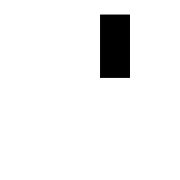
\includegraphics[width=\textwidth]{images/fingerprint_example.pdf}
\end{figure}
\begin{block}{Kernels used for the feature embedding in RankSVM}
\vspace{-0.25cm}
\begin{small}
\begin{itemize}
    \item Binary: Tanimoto kernel 
\begin{center}
    $\kmol(m_i,m_j)=\frac{b(m_i)^T b(m_j)}{b(m_i)^T b(m_i)+b(m_j)^T b(m_j)-b(m_i)^T b(m_j)}$
\end{center}
    \item Count: MinMax kernel 
\begin{center}
    $\kmol(m_i,m_j)=\frac{\sum_{s=1}^{N_{sub}}\min(c_s(m_i),c_s(m_j))}{\sum_{s=1}^{N_{sub}}\max(c_s(m_i),c_s(m_j))}$
\end{center}
\end{itemize}
\end{small}
\end{block}
}

\frame{ 
    \frametitle{Compare binary and counting molecular fingerprints}
%     \framesubtitle{Encoding molecular structures using MACCS dictionary molecular fingerprints.}

\begin{itemize}
    \item Pairwise prediction accuracy ($\pm 2\sigma$) for different target systems
    \item RankSVM models trained using single system $\Pref(\sys)$.
\end{itemize}

\begin{table}[!t]
\begin{tabular}{@{}lcc@{}}
    \toprule 
    Target system $\sys$ & Binary MACCS & Counting MACCS \\\midrule
    Eawag\_XBridgeC18 & $0.796 (\pm 0.015)$ & $\mathbf{0.844 (\pm 0.011)}$ \\
    FEM\_long         & $0.882 (\pm 0.016)$ & $\mathbf{0.905 (\pm 0.015)}$ \\
    RIKEN             & $0.826 (\pm 0.024)$ & $\mathbf{0.848 (\pm 0.017)}$ \\
    UFZ\_Phenomenex   & $0.790 (\pm 0.027)$ & $\mathbf{0.802 (\pm 0.017)}$ \\
    LIFE\_old         & $0.842 (\pm 0.050)$ & $\mathbf{0.862 (\pm 0.035)}$ \\
    \bottomrule
\end{tabular}
\end{table} 
}

\frame{
    \frametitle{Train model with preferences from different systems}
    \framesubtitle{Can pairwise predictor benefit from information of different systems?}

\begin{block}{Compare performance of different training sets}
\begin{itemize}
    \item Single system, target data only: $\Pref(\sys)$
    \item Multiple systems, \emph{no} target data: $\Pref\setminus\Pref(\sys)$
    \item Multiple systems, all available data: $\Pref$
    \item Varying percentage ???
\end{itemize}
\end{block}
\begin{block}{Comparison method}
\begin{itemize}
    \item Support Vector Regression (SVR) trained on retention times directly \cite{Aicheler2015}.
    \item In multiple system setting: Retention times are considered jointly.
\end{itemize}
\end{block}
}

\frame{
    \frametitle{Train model with preferences from different systems}
    \framesubtitle{Application setting: Training retention times only available from single target system.}
    
\begin{center}
    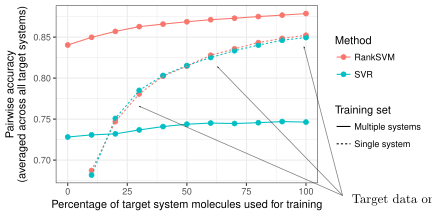
\includegraphics[width=\textwidth]{images/pwacc_2_marked_4.pdf}
\end{center}
\vspace{-0.25cm}
\begin{block}{Observations}
\begin{itemize}
    \item Increasing amount of training data improves prediction.
    \item RankSVM and SVR perform equally.
\end{itemize}
\end{block}
}

\frame{
    \frametitle{Train model with preferences from different systems}
    \framesubtitle{Application Setting: Training retention times only available \emph{from not target} system.}
    
\begin{center}
    \includegraphics[width=0.9\textwidth]{images/pwacc_2_marked_2.pdf}
\end{center}
\vspace{-0.25cm}
\begin{block}{Observations}
\begin{itemize}
    \item Performance of single system \emph{without} data from the target.
    \item RankSVM outperforms SVR by considering retention \emph{orders}.
\end{itemize}
\end{block}
}

\frame{
    \frametitle{Train model with preferences from different systems}
    \framesubtitle{Application Setting: Training retention times from target \emph{and} others systems available.}
    
\begin{center}
    \includegraphics[width=0.9\textwidth]{images/pwacc_2_marked_3.pdf}
\end{center}
\vspace{-0.25cm}
\begin{small}
\begin{block}{Observations}
\vspace{-0.15cm}
\begin{itemize}
    \item Considering target \emph{and} non-target systems' data outperforms single system.
    \item RankSVM again outperforms SVR.
\end{itemize}
\end{block}
\end{small}
}
